\newpage
\chapter{Architektura systemu}
\begin{figure}[!ht]
    \centering
    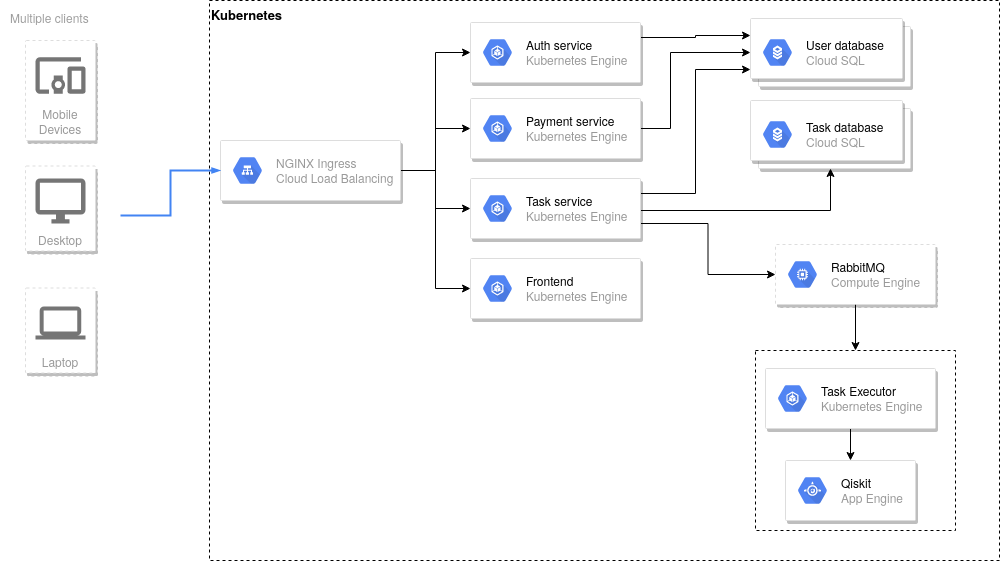
\includegraphics[width=\textwidth]{images/arch.png}
    \caption{Architektura systemu ROSA}
    \label{fig:sys_arch}
\end{figure}
\section{Ingress Controller}
Obiekt, który odpowiada za zarządzanie dostępem z zewnątrz klustera Kubernetes do serwisów działających wewnątrz klastra. Ingress odpowiada za równoważenie obciążenia oraz przekierowywanie zapytań dotyczących konkretnych serwisów zgodnie ze URI zapytań. W ramach systemu ROSA, zastosowano typ Nginx Ingress, który odpowiada za obsługę czterech serwisów wewnątrz klastra:
\begin{enumerate}
    \item Auth service - poprzez prefiks /auth
    \item Payment service - poprzez prefiks /payment
    \item Task service - poprzez prefiks /task
    \item Frontend - poprzez ścieżkę domyślną
\end{enumerate}
Dzięki wykorzystaniu elementu Ingress, całość systemu jest dostępna pod jednym adresem. Dodatkowo, pozostała część klastra jest całkowicie odseparowana, użytkownik może uzyskać do niej jedynie pośredni dostęp w postaci API udostępnionych serwisów.
\section{Frontend - Nginx}
Interfejs użytkownika jest generowany przy użyciu biblioteki Angular z użyciem języka TypeScript. Integracja z pozostałą częścią systemu odbywa się poprzez pozostałe serwisy i wysyłanie żądań na element Ingress.
\section{Auth service}
Auth service odpowiada za uwierzytelnianie użytkownika wykorzystując do tego standard JWT. Serwis udostępnia operacje:
\begin{itemize}
    \item rejestracji,
    \item logowania,
    \item pobierania danych użytkownika,
    \item zmiany danych użytkownika.
\end{itemize}
\section{Payment service}
Serwis ten używany jest w celu wygenerowania nowych zleceń doładowywania konta użytkownika. Obsługa płatności realizowana jest przez zewnętrzny systemem PayU. Payment service integruje się z tym systemem, poprzez system przekierowań oraz notyfikacji.
\section{Task service}
TODO Rafał Galczak/Wojciech Gruszka
\section{Bazy danych}
Dane przechowywane w systemie zostały podzielone między dwie bazy danych. Dane zostały podzielone na powiązane z użytkownikiem i powiązane z wykonywanymi wewnętrznie zadaniami. Na rysunku \ref{fig:db_model} przedstawiony został model baz danych.
\begin{figure}[!ht]
    \centering
    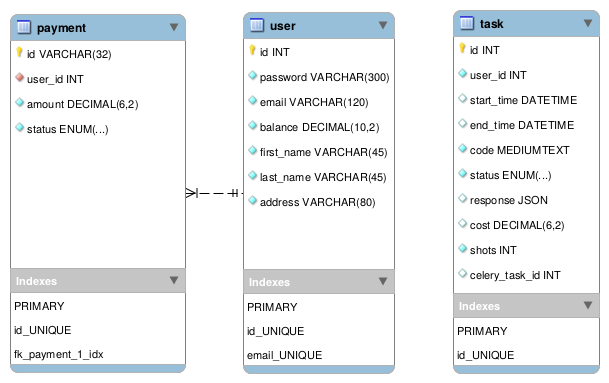
\includegraphics[width=\textwidth]{images/database.png}
    \caption{Model baz danych}
    \label{fig:db_model}
\end{figure}
Zastosowanie takiego podejścia i odseparowanie danych wrażliwych użytkownika umożliwia różny poziom zarządzania oraz pozwala zapewnić więszą niezawodność, nie powodując jednocześnie problemów z integralnością danych. Obywie bazy danych wykorzystują mechnizm replikacji.
\subsection{User database}
W pierwszej bazie przechowywane są wszelkie informacje dotyczące użytkowników. Składa się ona z dwóch tabel:
\begin{itemize}
    \item user - konta użytkowników wraz ze wszystkimi danymi wymaganymi do przeprowadzenia płatności,
    \item payment - zakończone lub obecnie przeprowadzane procesy płatności PayU.
\end{itemize}
\subsection{Task database}
TODO Rafał Galczak/Wojciech Gruszka
\section{RabbitMQ}
TODO Rafał Galczak/Wojciech Gruszka
\section{Task executor}
TODO Rafał Galczak/Wojciech Gruszka
\section{Qiskit}
TODO Rafał Galczak/Wojciech Gruszka
